\newpage
\section{Python}

\subsection{Gerencimaneto de pacote}

Python Package Index - PIP~\footnote{https://pypi.org/project/pip}
Sistema de gerenciamento de pacotes padrão de facto usado para instalar e gerenciar pacotes de software escritos em Python. 
Muitos pacotes podem ser encontrados na fonte padrão para pacotes e suas dependências.

Anaconda~\footnote{https://www.anaconda.com} 
Distribuição gratuita e de código aberto das linguagens de programação Python e R para computação científica, que visa simplificar o gerenciamento e a implantação de pacote.

Conda~\footnote{https://docs.conda.io/en/latest}
Gerenciador de pacotes e sistema de gerenciamento de ambiente de código aberto, plataforma cruzada e independente de linguagem.


\subsection{Essencial}

NumPy é um pacote para a linguagem Python que suporta arrays e matrizes multidimensionais, possuindo uma larga coleção de funções matemáticas para trabalhar com estas estruturas.

\begin{figure}[!htp]
    \centering
    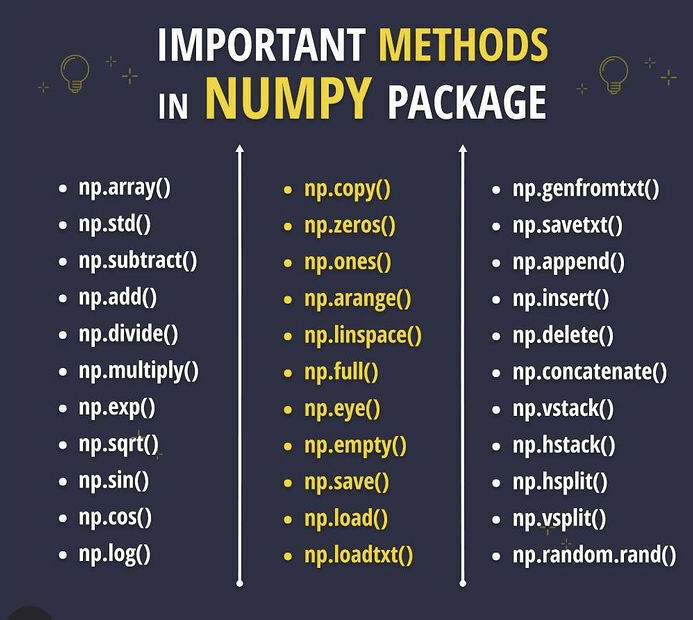
\includegraphics[scale=.9]{../img/python/numpy.jpeg}
    \caption{NumPy}
    \label{img:numpy}
\end{figure}

Pandas é uma biblioteca de software criada para a linguagem Python para manipulação e análise de dados. 
Em particular, oferece estruturas e operações para manipular tabelas numéricas e séries temporais. 
O nome é derivado de painel data.

\begin{figure}[!htp]
    \centering
    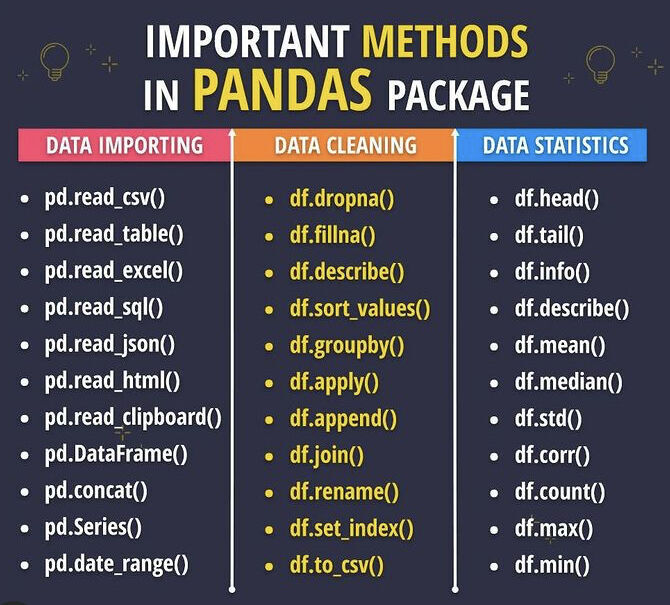
\includegraphics[scale=.9]{../img/python/pandas.jpeg}
    \caption{Pandas}
    \label{img:pandas}
\end{figure}

\subsection{Matemática}

SymPy é uma biblioteca Python para computação simbólica. 
Ela fornece ferramentas de álgebra computacional tanto como uma aplicação independente como, também, uma biblioteca para outras aplicações.

SciPy é uma biblioteca Open Source em linguagem Python que foi feita para matemáticos, cientistas e engenheiros. 
Também tem o nome de uma popular conferência de programação científica com Python.

Statsmodels é um pacote Python que permite aos usuários explorar dados, estimar modelos estatísticos e executar testes estatísticos

\subsection{Visualização de dados}

Matplotlib \footnote{https://matplotlib.org/} é uma biblioteca para geração de gráficos e visualizações de dados em geral, feita para e da linguagem de programação Python e sua extensão de matemática NumPy.

\begin{figure}[!htp]
    \centering
    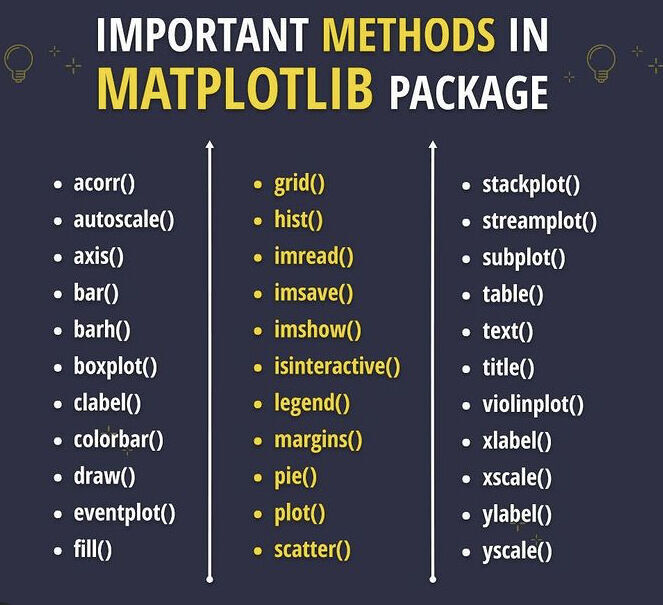
\includegraphics[scale=.9]{../img/python/matplotlib.jpeg}
    \caption{Matplotlib}
    \label{img:matplotlib}
\end{figure}

Seaborn~\footnote{https://seaborn.pydata.org/}
\begin{figure}[!htp]
    \centering
    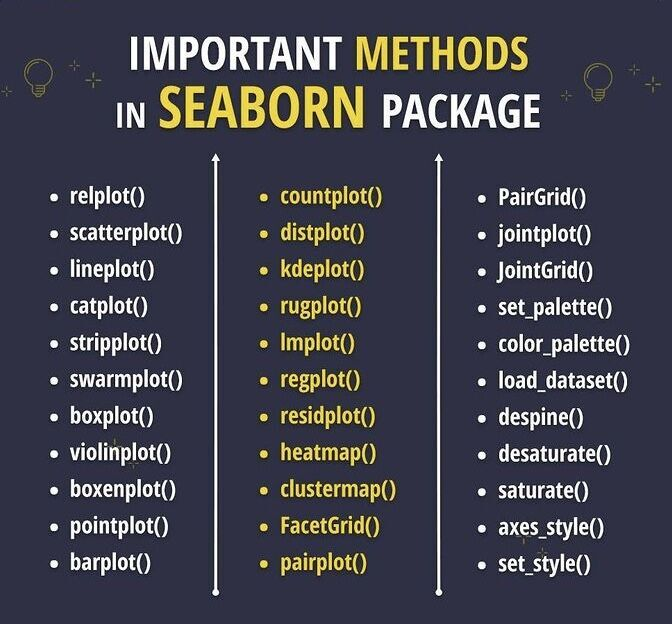
\includegraphics[scale=.5]{../img/python/seaborn.jpeg}
    \caption{Seaborn}
    \label{img:seaborn}
\end{figure}


\subsection{Web Scraping}

LXML~\footnote{https://lxml.de}

HTLM5LIB~\footnote{https://html5lib.readthedocs.io/en/latest}

Beautiful Soup~\footnote{https://www.crummy.com/software/BeautifulSoup/bs4/doc}

\subsection{Aprendizagem de máquina}

Scikit-learn~\footnote{https://scikit-learn.org}
Biblioteca de aprendizado de máquina de código aberto para a linguagem de programação Python

TensorFlow~\footnote{https://www.tensorflow.org}
Biblioteca de código aberto para aprendizado de máquina aplicável a uma ampla variedade de tarefas. 
É um sistema para criação e treinamento de redes neurais para detectar e decifrar padrões e correlações

Keras~\footnote{https://keras.io}
Biblioteca de rede neural de código aberto escrita em Python. 
Ele é capaz de rodar em cima de TensorFlow, Microsoft Cognitive Toolkit, R, Theano, ou PlaidML. 
Projetado para permitir experimentação rápida com redes neurais profundas, ele se concentra em ser fácil de usar, modular e extensível

\subsection{Processamento de imagens}

Python Imaging Library
Biblioteca da linguagem de programação Python que adiciona suporte à abertura e gravação de muitos formatos de imagem diferentes.

OpenCV
Biblioteca multiplataforma, totalmente livre ao uso acadêmico e comercial, para o desenvolvimento de aplicativos na área de Visão computacional

Scikit-image
Biblioteca de processamento de imagens de código aberto para a linguagem de programação Python. Inclui algoritmos para segmentação, transformações geométricas, manipulação do espaço de cores, análise, filtragem, morfologia, detecção de recursos e muito mais.

PyTorch
Biblioteca de aprendizado de máquina de código aberto baseada na biblioteca Torch, usada para aplicativos como visão computacional e processamento de linguagem natural